\documentclass{article}
\usepackage{CJKutf8}
\usepackage{graphicx}
\usepackage{fancyhdr}
\usepackage{cite}
\usepackage{amsmath}
\usepackage[framed,numbered,autolinebreaks,useliterate]{mcode}

\pagestyle{fancy}
\fancyhead[L]{202013407457}

\title{Digital Image Processing - HW1}
\author{杜睿 教学班1294}
\date{\today}

\begin{document}
\begin{CJK}{UTF8}{gbsn}
\maketitle{}

\section{Problem 1}

Please give the transform equation, which can reduce the gray range $[0, 120]$ to $[0, 40]$,
and change the gray range $[120, 200]$ to $[40, 200]$, and the gray range $[200, 255]$ to $[200, 255]$. Then please give the MATLAB function code to complete the contrast enhancement\cite{19b2749cc0f95d6522a84a3039aea315d92ae9fb}. They both are uint8 class.

{\centering
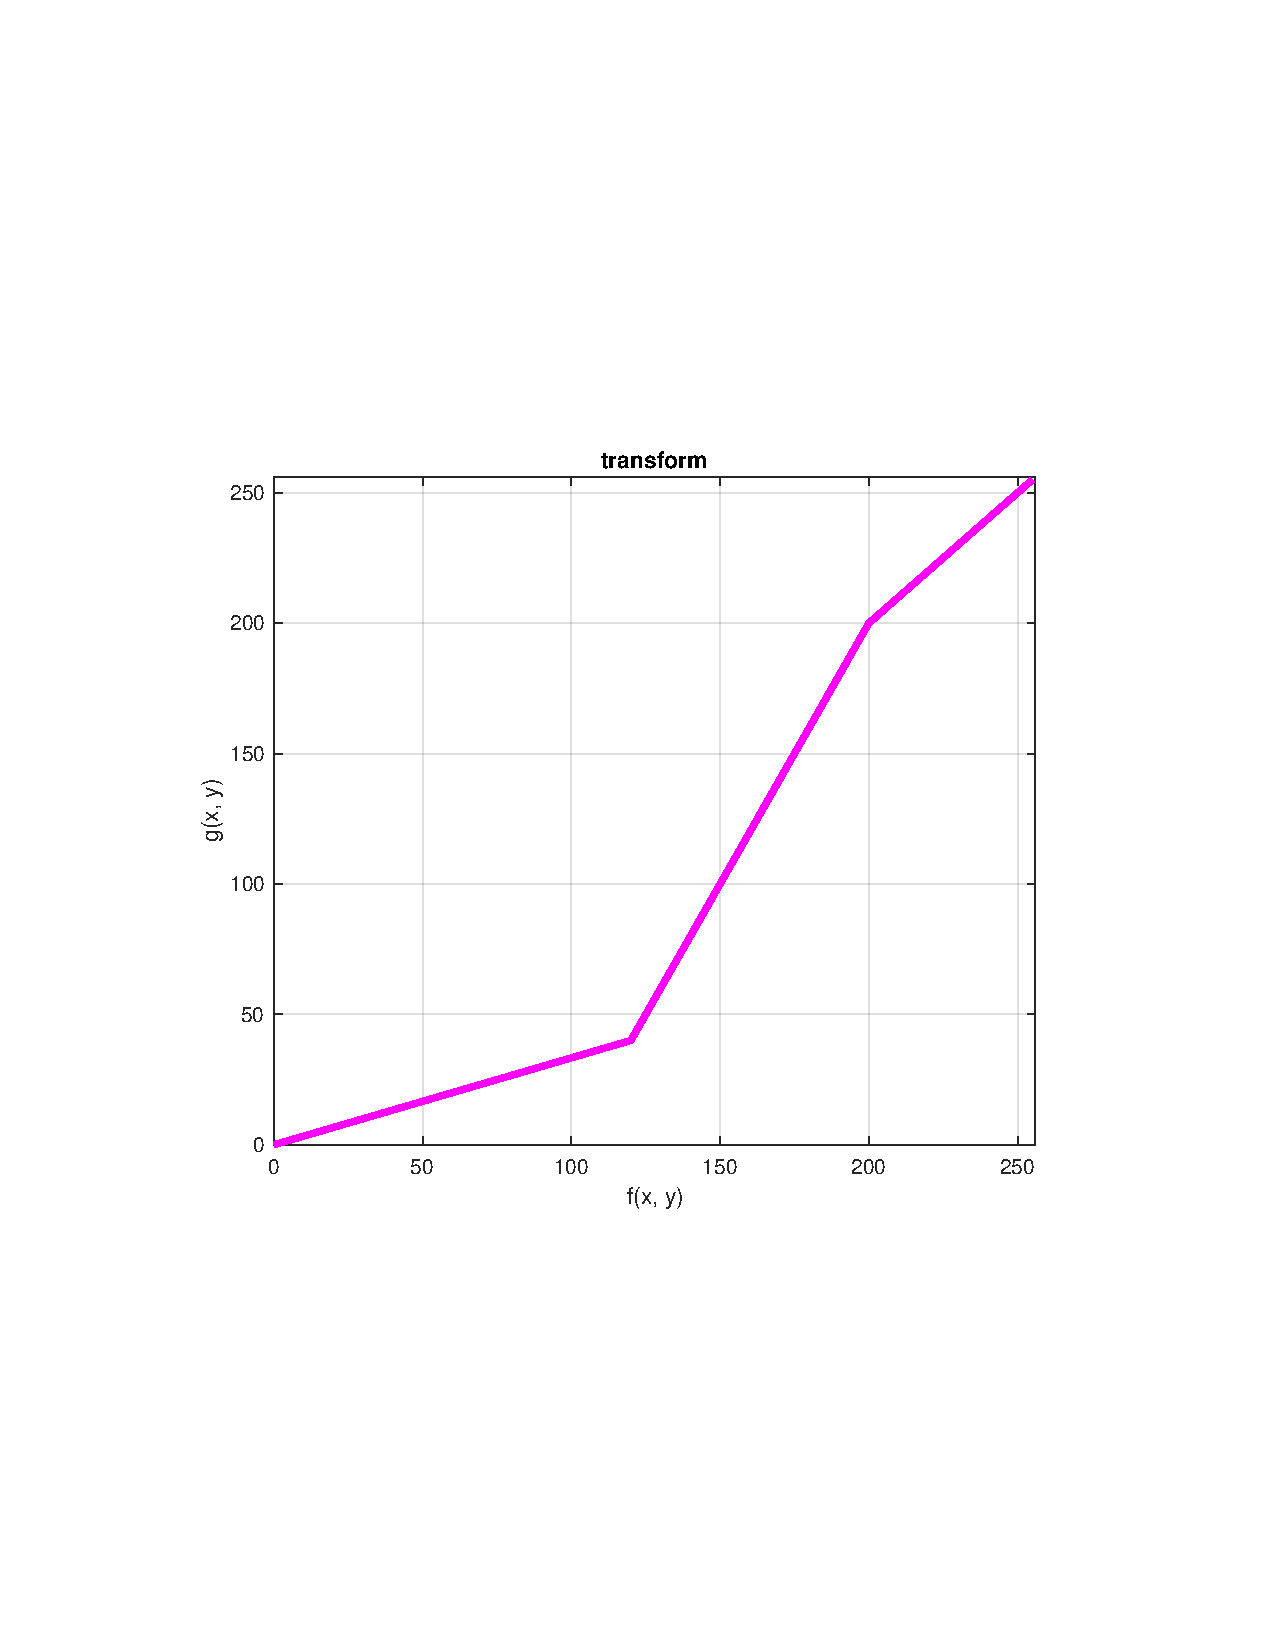
\includegraphics[width=1\textwidth]{transform.pdf}}

\begin{lstlisting}
img=imread('bubbles.tif')
imshow(img)

g=@(f) (f>=0&f<120).*f.*1/3 + (f>=120&f<200).*(2.*f-200) + (f>=200&f<256).*f

converted=uint8(g(double(img)))
imshow(converted)

\end{lstlisting}

\section{Problem 2}

Please give the self-defining code of an m-file with MATLAB program language,  which can show the 256 gray levels’ histogram of an input image \textbf{without} using the image processing function ‘imhist’. The result is a row vector. Let the image is ‘rice.tif’ with uint8 class data in the current folder.

\begin{lstlisting}
I=imread('rice.tif')
G=selfhist(I,256)
figure,bar(0:255,G)

function G=selfhist(I,T)
G=zeros(1,T);
for K = 0:255
    G(K+1)=sum(sum(I==K));
end
end
\end{lstlisting}

{\centering
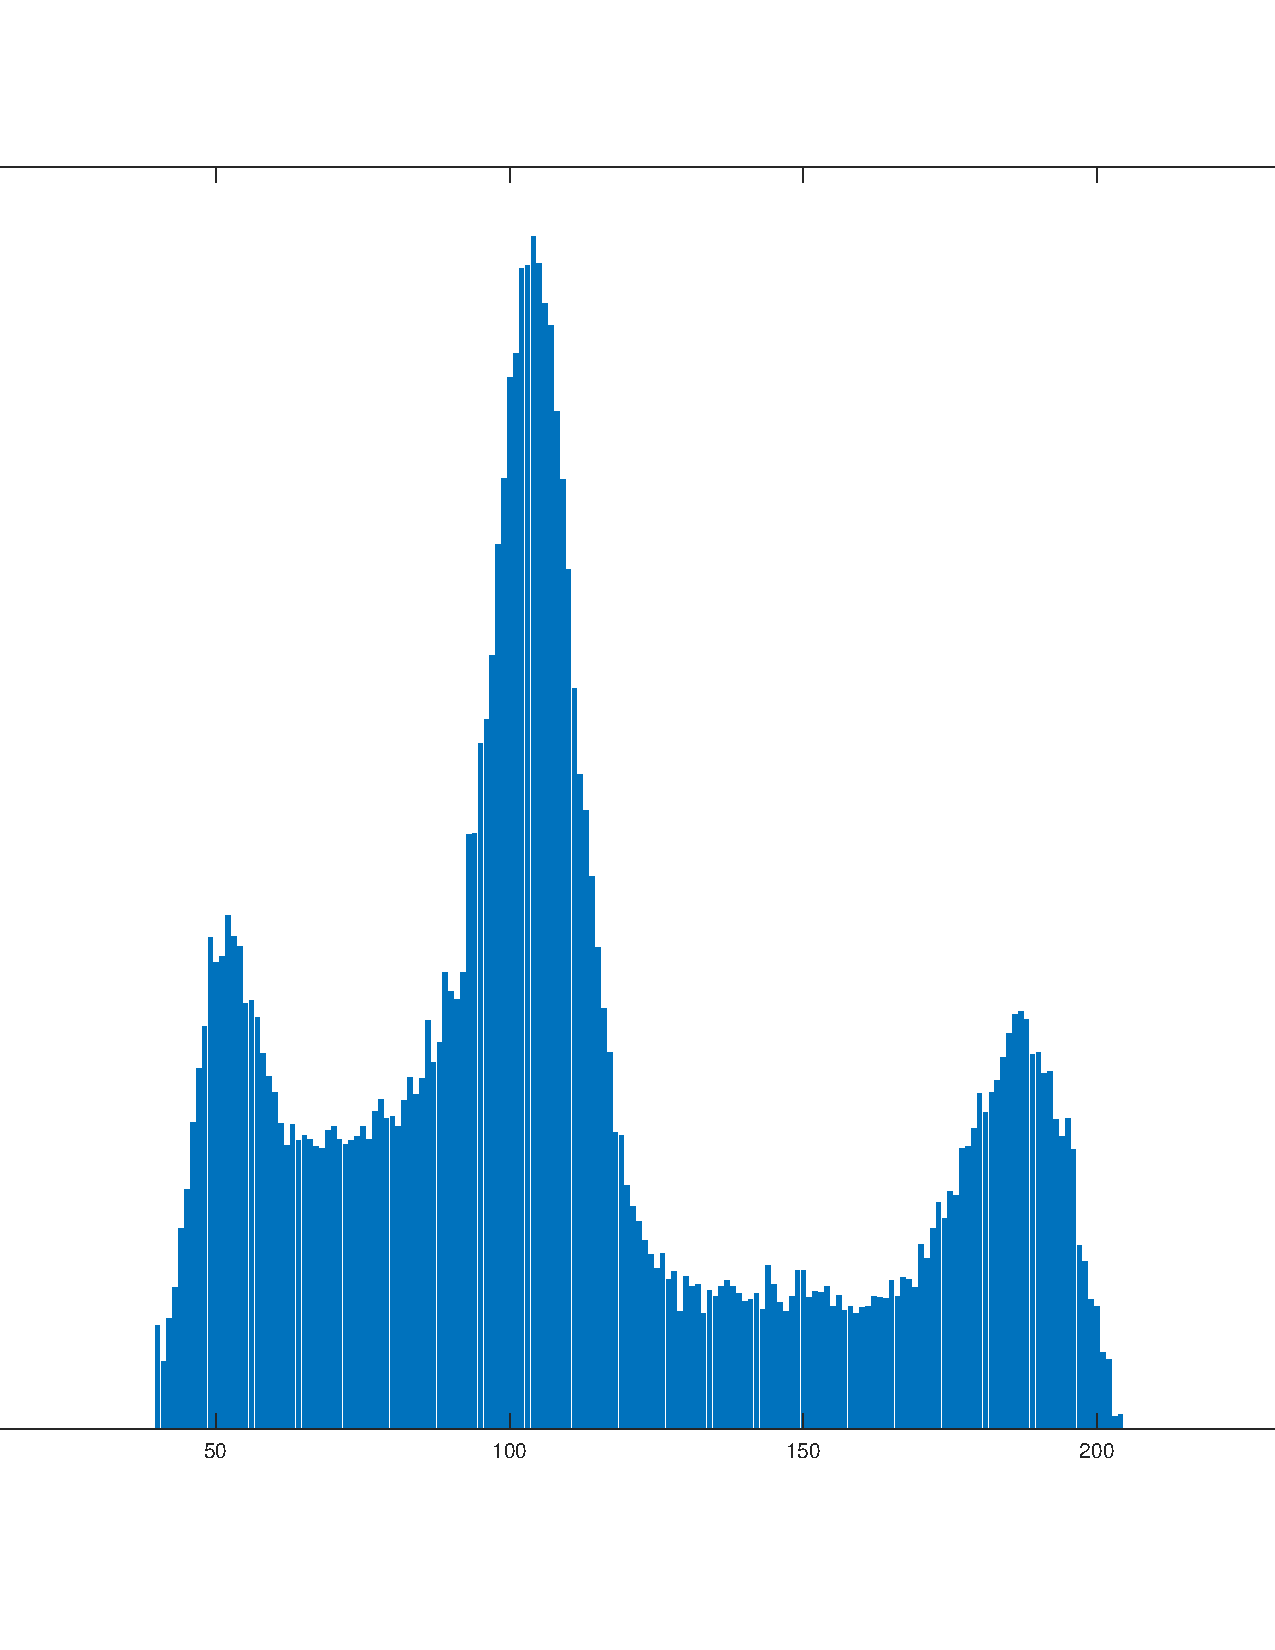
\includegraphics[width=1.0\textwidth,height=0.9\textwidth]{selfhist.pdf}}


\section{Problem 3}

{\centering
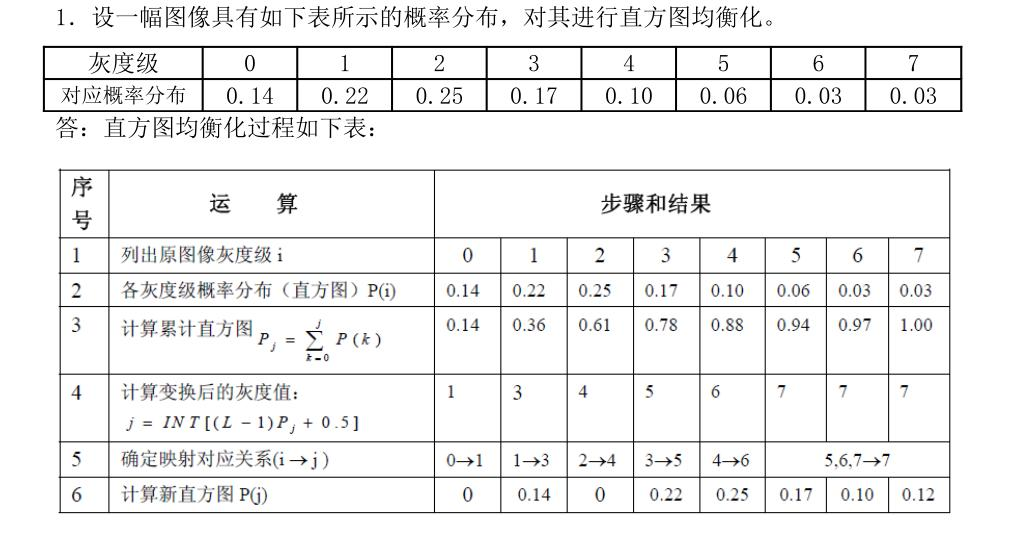
\includegraphics[width=0.8\textwidth,height=0.5\textwidth]{p3_key.jpg}}

jjj

\bibliographystyle{ieeetr}
\bibliography{TDNN.bib}


\end{CJK}
\end{document}